\section{State Estimation using a Kalman filter}

\subsection{} % a
The $\mathbf{Q}$ matrix is the process noise covariance matrix, which describes the covariance of the noise associated with the process itself.  The $\mathbf{R}$ matrix is the measurement, or observation, noise, which is associated with the noise which is introduced when a measurement is made. Finally, the $\mathbf{P}$ matrix is the estimation covariance, the covariance, or uncertainty of the given estimate.

% dimensions
All these matrices are square. The $\mathbf{Q}$ matrix has dimension according to the estimated state vector in our kalman filter, which in thise case makes it 4-by-4. The $R$ matrix likewise corresponds to the output vector and is hence 2-by-2. The covariance matrix $\mathbf{P}$ also corresponds to the state dimension and so is 4-by-4.

\subsection{} % b
MEMS rate gyros are the standard measurement devices for roll rate and yaw rate. These measurements can be modelled, as from \cite[p. 125]{beard_mclain_2012}, as \eqref{eq:gyro_model}. The parameters $k$ and $\beta$ are usually found experimentally to ensure that they are accurate, as they often are dependent on influences like temperature. $\eta$ is assumed to be zero-mean Gaussian noise. 

\begin{equation}
    \label{eq:gyro_model}
    \Upsilon_{\text{gyro}} = k_{\text{gyro}} \Omega + \beta_{\text{gyro}} + \eta_{\text{gyro}}'
\end{equation}

The types of noise which may affect a real system would usually be mechanical or electrical, like vibrations on the system and electro-magnetic noise on the measurement device. 

The white noise assumption in the Kalman filter would obviously be a problem if the noise wasn't white. This would mean that the filter would try to fit the measurement to a wrong noise-model, and therefore the estimate would not \textit{necessarily} converge to the correct value. 

% BEARD page 124

% Typical measurement model for the sensor

% What kind of noise would the sensor be affected by

% Example of a situation where white noise assumption may be problematic

\subsection{} % c
The Kalman filter is the optimal linear state estimator when the model perfectly models the real system, the noise is entirely white. uncorrelated with other noise or signals. Like mentioned in the previous subtask, we cannot generally assume the noise to be white for real life systems. For this simulation however, the generated noise is white, so in this case that assumption holds. Moreover, the model rarely depicts reality perfectly. The parameters are seldom known, and might even depend on environmental effects like wind and weather. Real systems also tend to have unmodeled dynamics, often non-linear, that we cannot capture in the linear model. In this case, we do have such unmodeled dynamics as the aileron dynamics (equation (3) in the assignment) are not modeled in the Kalman filter.

\subsection{} % d
The Kalman filter was implemented as a Matlab function according to the specifications found on BlackBoard. 

\subsection{} % e
See \figref{fig:3e}. 

\begin{figure}[ht]
	\centering
	\begin{subfigure}[b]{0.45\textwidth}
		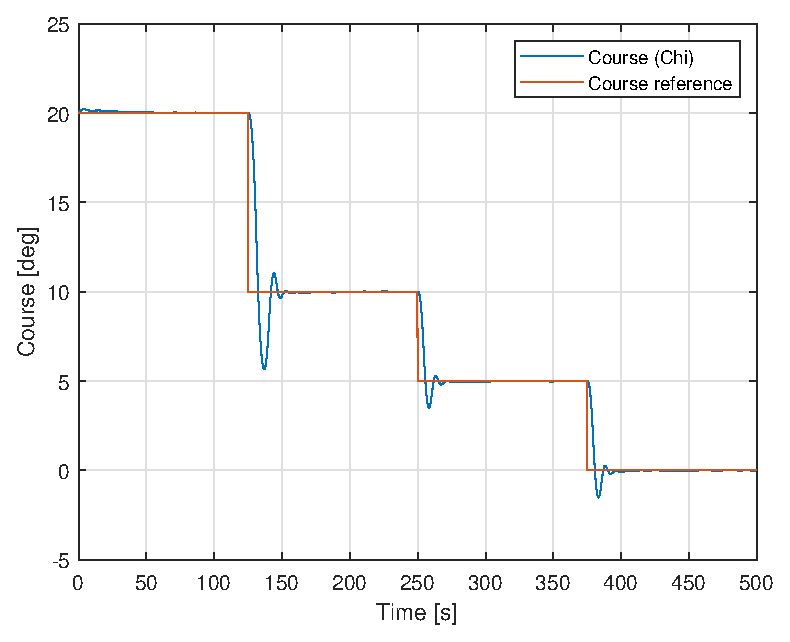
\includegraphics[width=\textwidth]{figures/3e/chi_course.eps}
		\caption{Course and desired course. }
		\label{fig:3e_chi_course}
	\end{subfigure}
	\begin{subfigure}[b]{0.45\textwidth}
		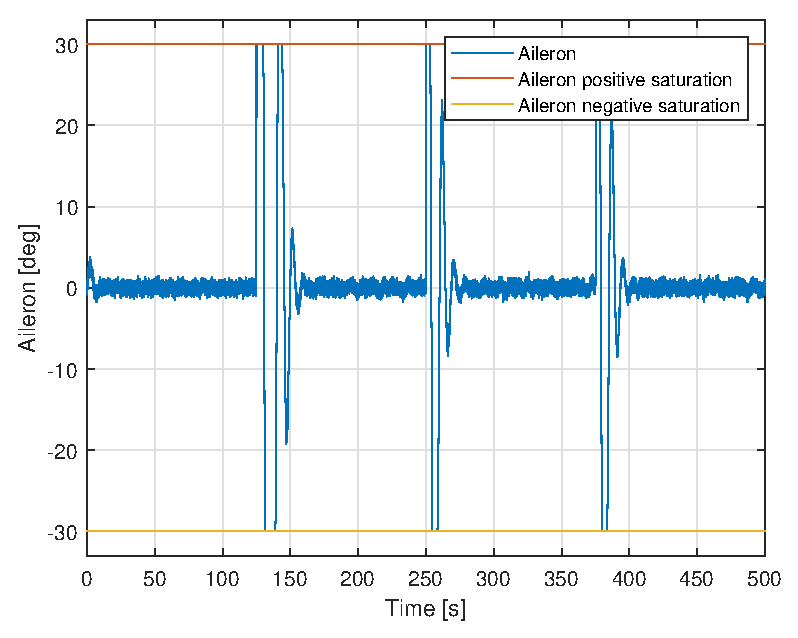
\includegraphics[width=\textwidth]{figures/3e/delta_a_aileron.eps}
		\caption{Aileron input. }
		\label{fig:3e_delta_a_aileron}
	\end{subfigure}
	\begin{subfigure}[b]{0.45\textwidth}
		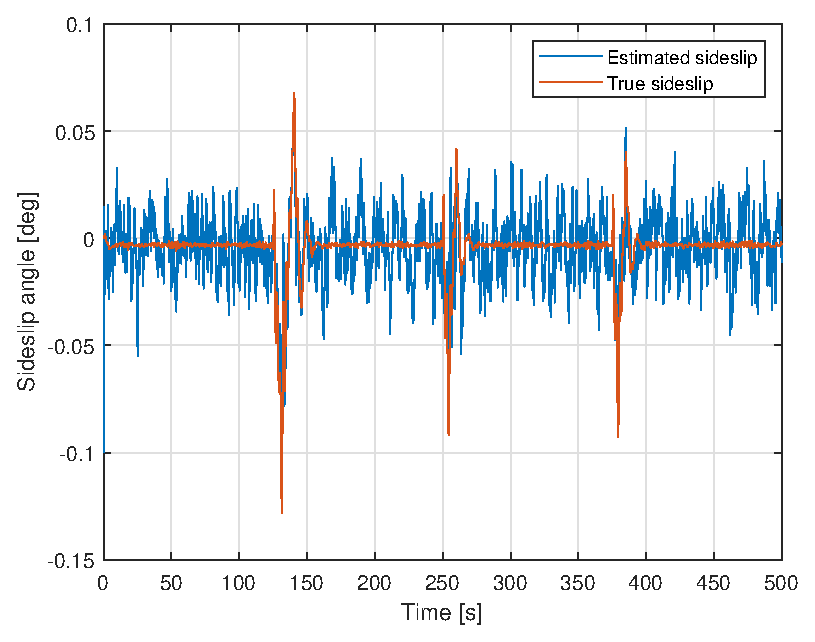
\includegraphics[width=\textwidth]{figures/3e/beta_sideslip.eps}
		\caption{Estimated and true sideslip. }
		\label{fig:3e_beta_sideslip}
	\end{subfigure}
	\begin{subfigure}[b]{0.45\textwidth}
		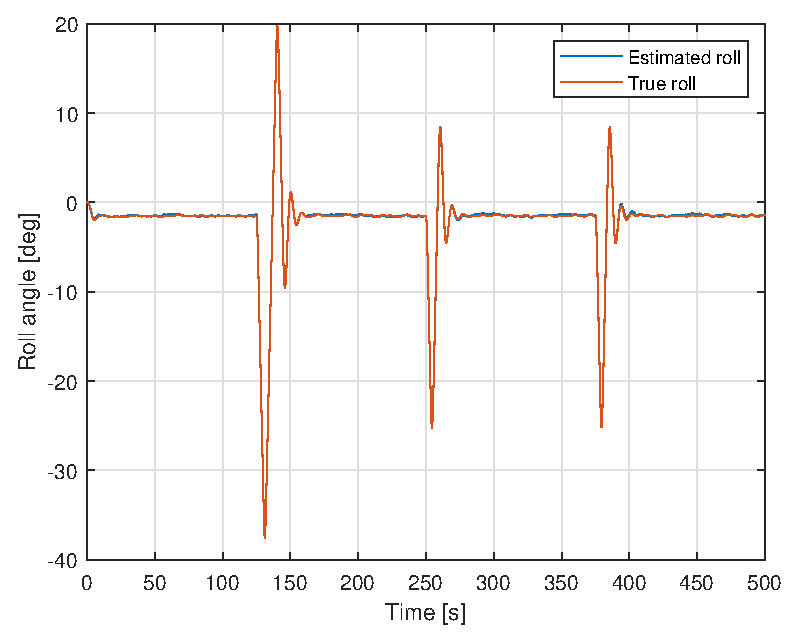
\includegraphics[width=\textwidth]{figures/3e/roll_phi.eps}
		\caption{Estimated and true roll angle. }
		\label{fig:3e_roll_angle}
    \end{subfigure}	
    \begin{subfigure}[b]{0.45\textwidth}
		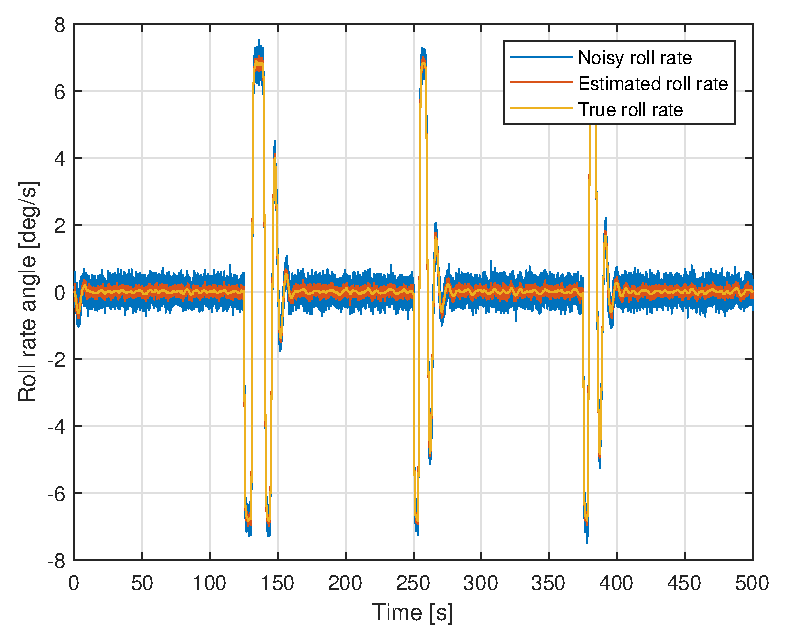
\includegraphics[width=\textwidth]{figures/3e/roll_rate_p.eps}
		\caption{Noisy, true and estimated roll rate. }
		\label{fig:3e_roll_rate_p}
	\end{subfigure}
	\begin{subfigure}[b]{0.45\textwidth}
		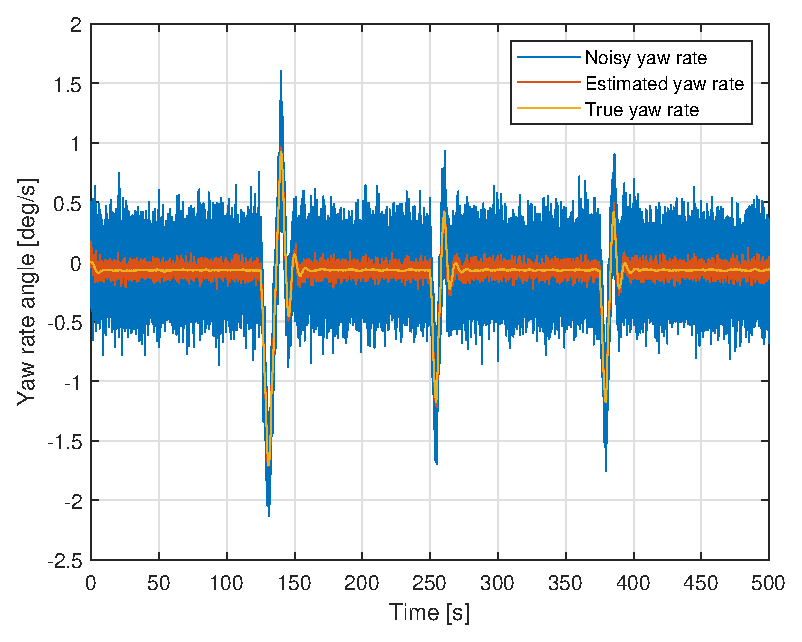
\includegraphics[width=\textwidth]{figures/3e/yaw_rate_r.eps}
		\caption{Noisy, true and estimated yaw rate. }
		\label{fig:3e_yaw_rate_r}
	\end{subfigure}
	\caption{Figures for task 3e)}\label{fig:3e}
\end{figure}

\subsection{} % f
See \figref{fig:3f}. The problem when using the noisy measurement directly is that the measurement (and the noise) is immediately introduced into the control system. The Kalman filter helps mitigate this, as we can see in the aileron inputs. With the noisy measurements directly inserted as in \figref{fig:3e}, the measurement noise gets propagated into the input, however with the Kalman filter, this noise is heavily decreased.

% comment on the preformance of the course control

% better? yes

% theoretical: bandwidth of the estimator compared to the control loop

\begin{figure}[ht]
	\centering
	\begin{subfigure}[b]{0.45\textwidth}
		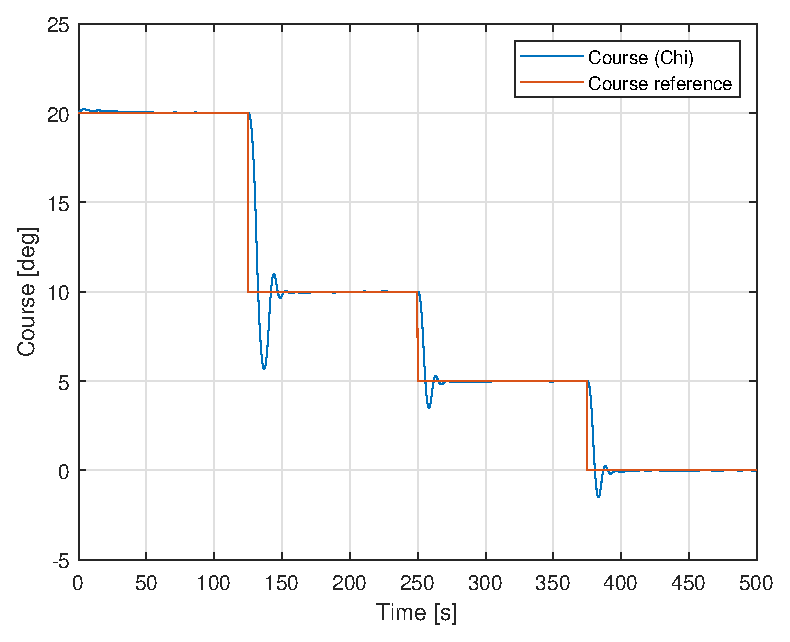
\includegraphics[width=\textwidth]{figures/3f/chi_course.eps}
		\caption{Course and desired course. }
		\label{fig:3f_chi_course}
	\end{subfigure}
	\begin{subfigure}[b]{0.45\textwidth}
		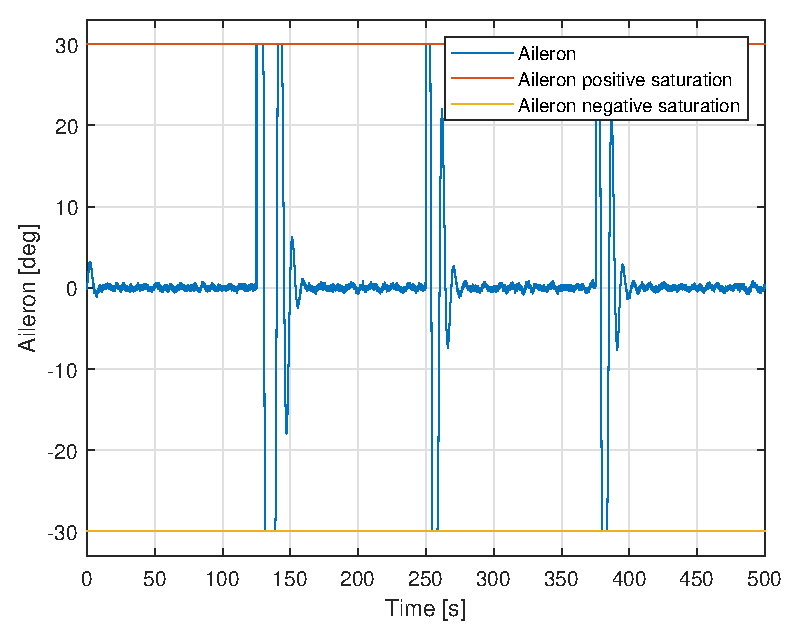
\includegraphics[width=\textwidth]{figures/3f/delta_a_aileron.eps}
		\caption{Aileron input. }
		\label{fig:3f_delta_a_aileron}
	\end{subfigure}
	\begin{subfigure}[b]{0.45\textwidth}
		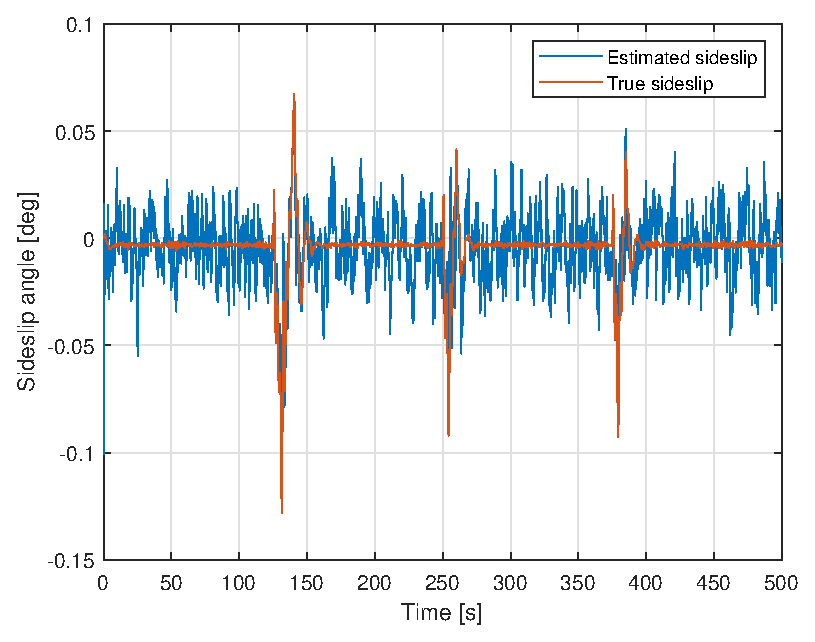
\includegraphics[width=\textwidth]{figures/3f/beta_sideslip.eps}
		\caption{Estimated and true sideslip. }
		\label{fig:3f_beta_sideslip}
	\end{subfigure}
	\begin{subfigure}[b]{0.45\textwidth}
		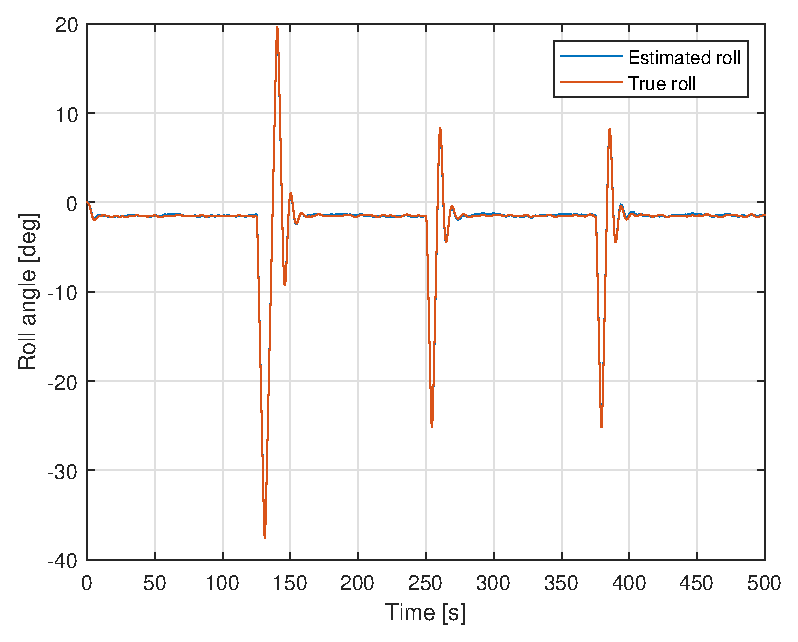
\includegraphics[width=\textwidth]{figures/3f/roll_phi.eps}
		\caption{Estimated and true roll angle. }
		\label{fig:3f_roll_angle}
    \end{subfigure}	
    \begin{subfigure}[b]{0.45\textwidth}
		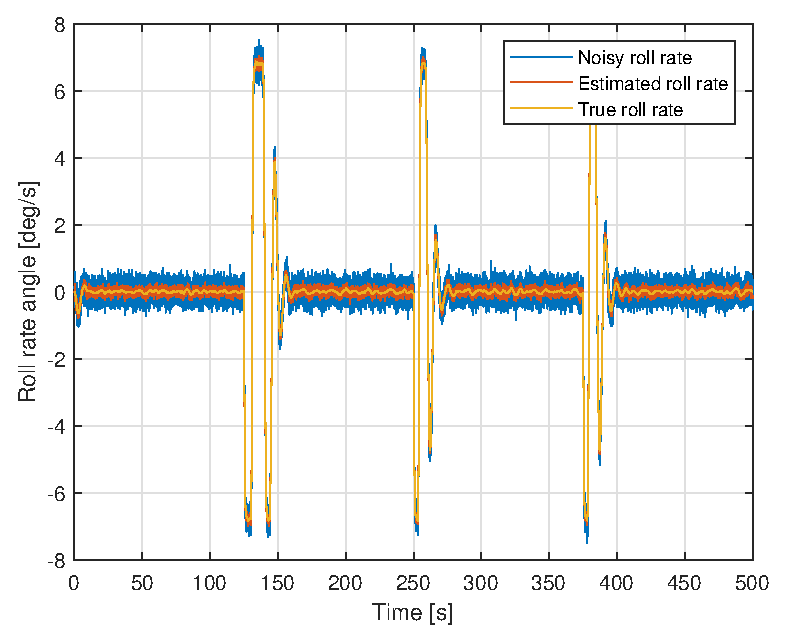
\includegraphics[width=\textwidth]{figures/3f/roll_rate_p.eps}
		\caption{Noisy, true and estimated roll rate. }
		\label{fig:3f_roll_rate_p}
	\end{subfigure}
	\begin{subfigure}[b]{0.45\textwidth}
		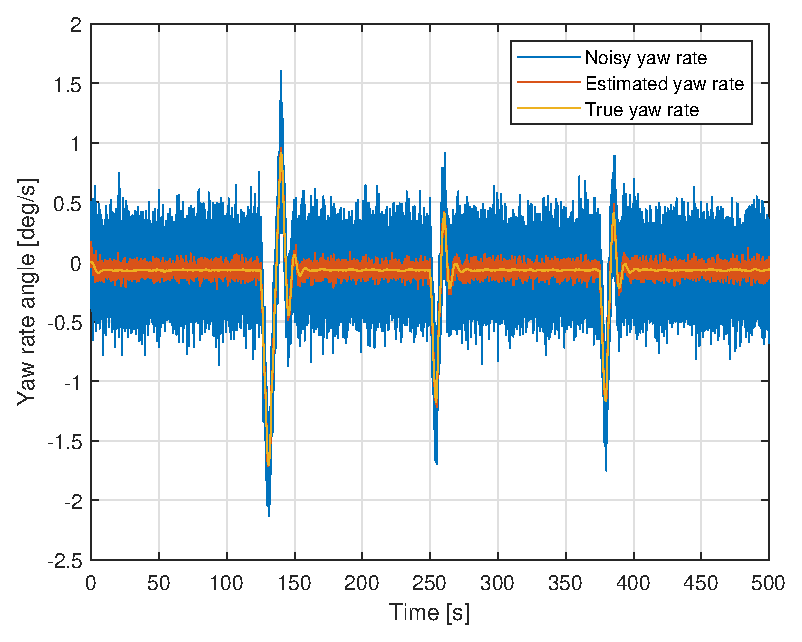
\includegraphics[width=\textwidth]{figures/3f/yaw_rate_r.eps}
		\caption{Noisy, true and estimated yaw rate. }
		\label{fig:3f_yaw_rate_r}
	\end{subfigure}		
	\caption{Figures for task 3f)}\label{fig:3f}
\end{figure}

\subsection{} % g
% should be some drift in the system, needed to decrease the number of steps to see. 

\figref{fig:3g}
\begin{figure}[ht]
	\centering
	\begin{subfigure}[b]{0.45\textwidth}
		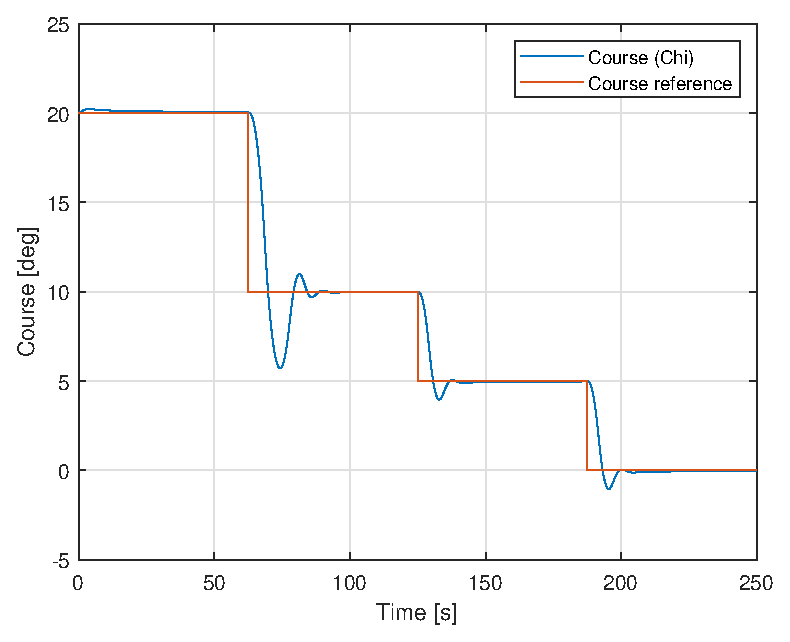
\includegraphics[width=\textwidth]{figures/3g/chi_course.eps}
		\caption{Course and desired course. }
		\label{fig:3g_chi_course}
	\end{subfigure}
	\begin{subfigure}[b]{0.45\textwidth}
		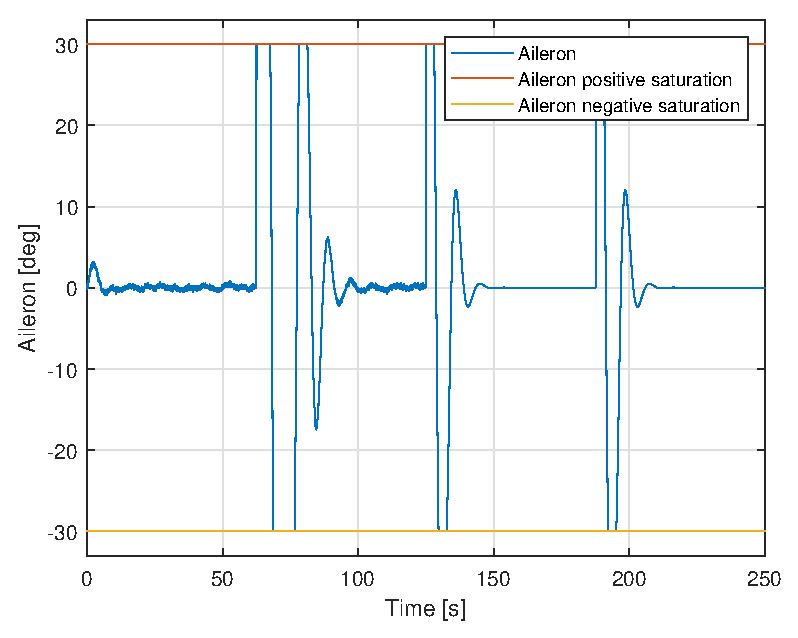
\includegraphics[width=\textwidth]{figures/3g/delta_a_aileron.eps}
		\caption{Aileron input. }
		\label{fig:3g_delta_a_aileron}
	\end{subfigure}
	\begin{subfigure}[b]{0.45\textwidth}
		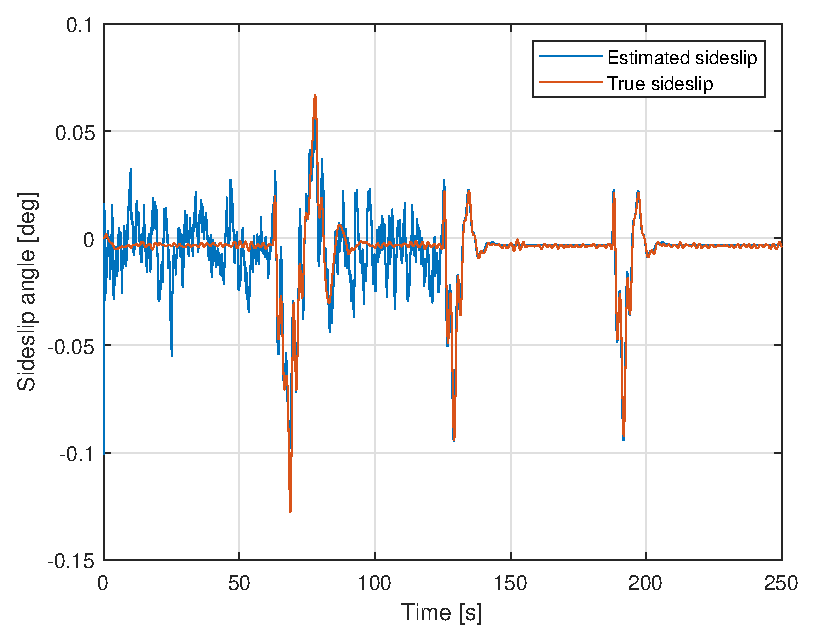
\includegraphics[width=\textwidth]{figures/3g/beta_sideslip.eps}
		\caption{Estimated and true sideslip. }
		\label{fig:3g_beta_sideslip}
	\end{subfigure}
	\begin{subfigure}[b]{0.45\textwidth}
		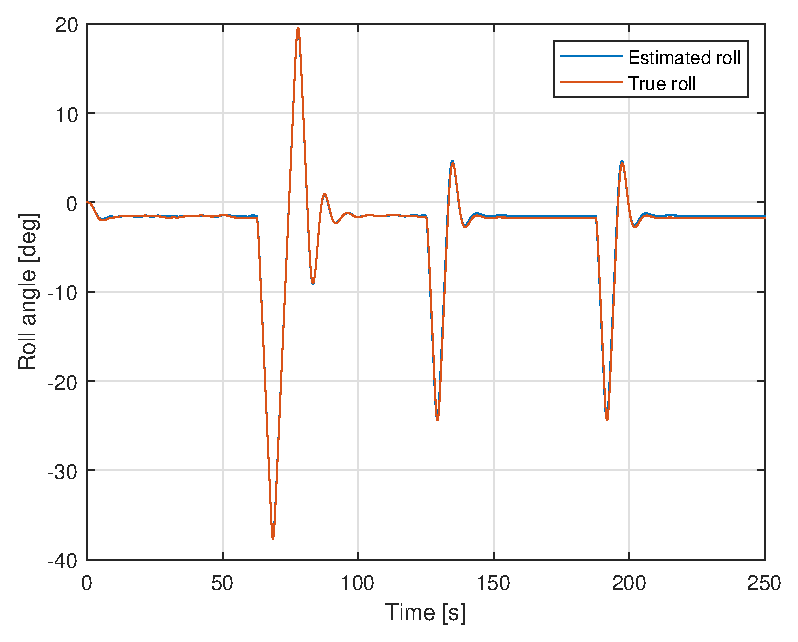
\includegraphics[width=\textwidth]{figures/3g/roll_phi.eps}
		\caption{Estimated and true roll angle. }
		\label{fig:3g_roll_angle}
    \end{subfigure}	
    \begin{subfigure}[b]{0.45\textwidth}
		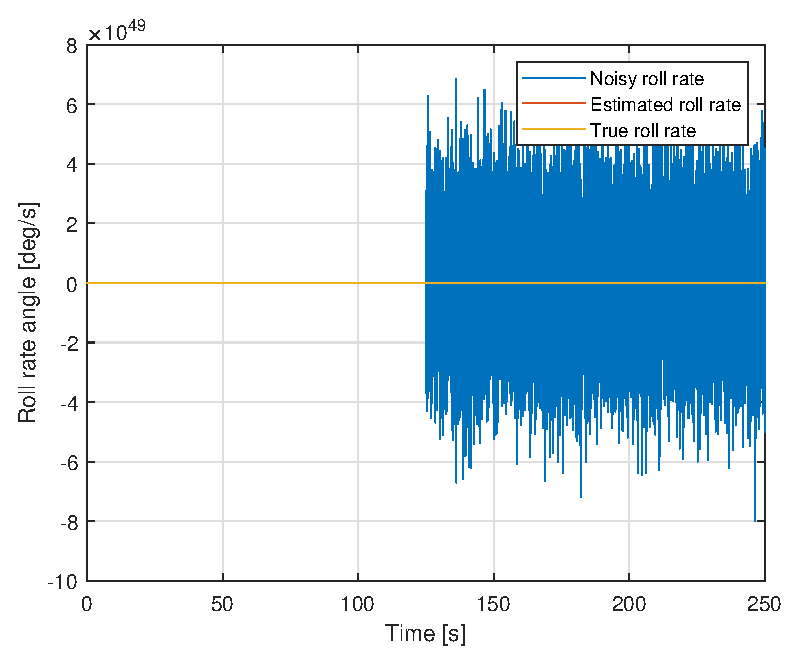
\includegraphics[width=\textwidth]{figures/3g/roll_rate_p.eps}
		\caption{Noisy, true and estimated roll rate. }
		\label{fig:3g_roll_rate_p}
	\end{subfigure}
	\begin{subfigure}[b]{0.45\textwidth}
		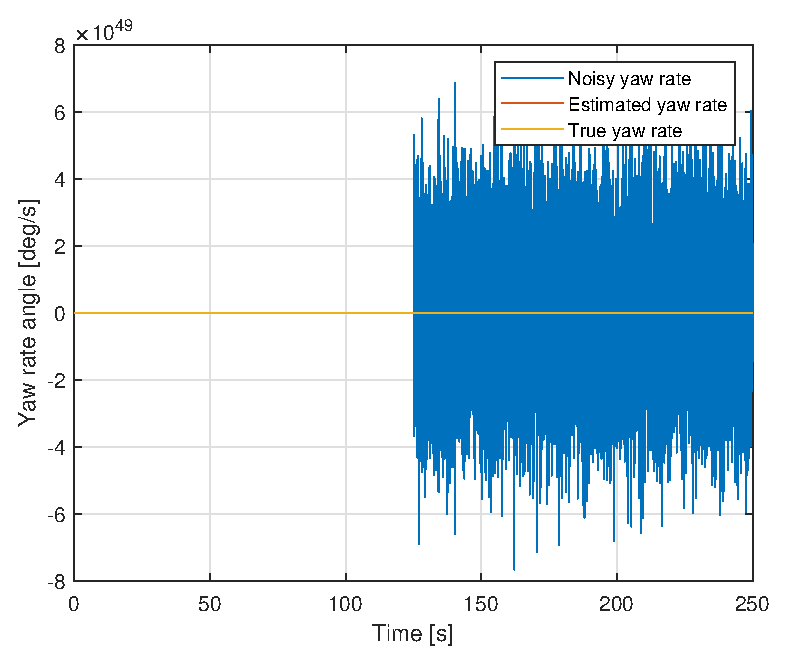
\includegraphics[width=\textwidth]{figures/3g/yaw_rate_r.eps}
		\caption{Noisy, true and estimated yaw rate. }
		\label{fig:3g_yaw_rate_r}
	\end{subfigure}		
	\caption{Figures for task 3g)}\label{fig:3g}
\end{figure}
